\section{Auswertung}

\subsection{Bestimmung der Reichweite und des Energieverlustes von Alpha-Strahlung}

\subsubsection{Messung 1 - $d = \SI{23}{\mm}$ \label{sec:23mm}}

In Tabelle \ref{tab:reich23mm} befinden sich die aufgenommenen Messwerte.
\begin{table}[H]
   \centering
   \caption{Aufgenommene Messwerte im Abstand $d = \SI{23}{\mm}$ }
   \label{tab:reich23mm}
   \begin{tabular} { c c c }
 \toprule
 {$p\:/\: \mathrm{mbar}$} & {$N$} & {Channel} \\
    \midrule
    0 & 82567 & 1127 \\
    50 & 58847 & 1088 \\
    100 & 57532 & 1045 \\
    150 & 57965 & 1022 \\
    200 & 56132 & 970 \\
    250 & 56827 & 934 \\
    300 & 56955 & 932 \\
    350 & 53724 & 857 \\
    400 & 54801 & 858 \\
    450 & 53282 & 819 \\
    500 & 47913 & 747 \\
    550 & 43768 & 699 \\
    600 & 39368 & 666 \\
    650 & 35751 & 625 \\
    700 & 37637 & 614 \\
    \bottomrule
  \end{tabular}
\end{table}


Der effektive Abstand $x$ zwischen Strahler und Detektor ergibt sich aus Gleichung \eqref{eqn:xeff}.
\begin{equation}
  x = x_0 \cdot \frac{p}{p_0}
  \label{eqn:xeff}
\end{equation}
\begin{center}
  \tiny{($p_0 = \SI{1013}{\milli \bar} \: \hat{=} \: \text{Normaldruck}$)}
\end{center}

In Abbildung \ref{fig:reich23mm} sind die Zählraten in Abhängigkeit vom effektiven Abstand aufgetragen.
Dabei wird der Messwert bei $p = \SI{0}{\milli \bar}$ weggelassen, da er so stark von den restlichen Werten abweicht, dass er die nachfolgende
Auswertung verfälschen würde.
\begin{figure}[H]
  \centering
  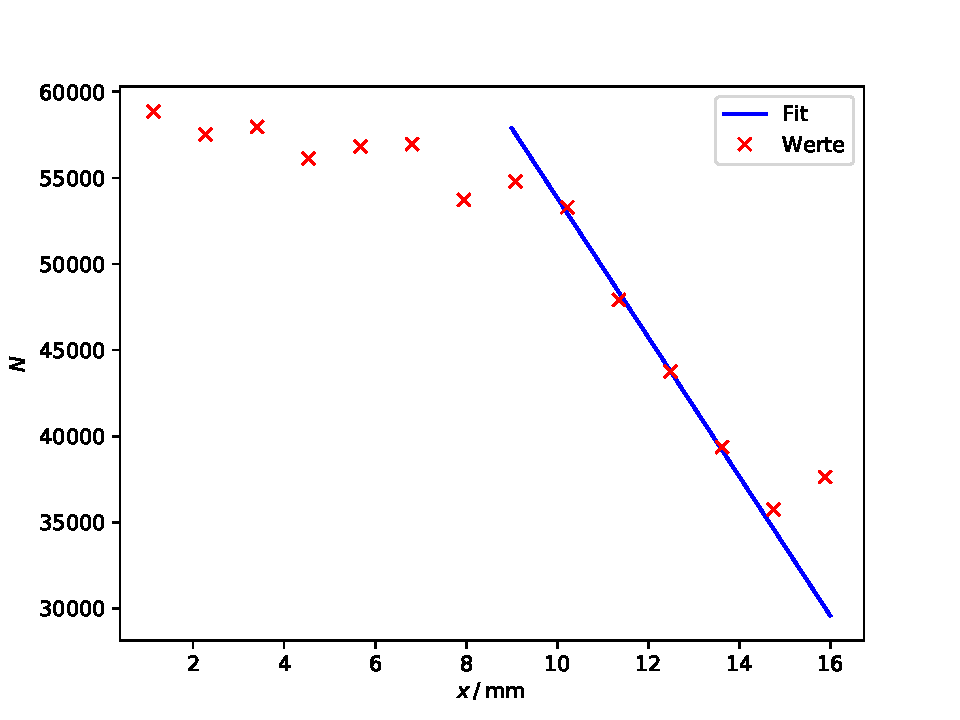
\includegraphics[width=\textwidth]{Plots/reich23mm.pdf}
  \caption{$N$-$x$-Diagramm zur Bestimmung der mittleren Reichweite von $\symup{\alpha}$-Strahlung}
  \label{fig:reich23mm}
\end{figure}

Eine lineare Regression $f(x) = -a \cdot x + b$ ergibt
\begin{align*}
  a &= \SI{4,0(2)e3}{\per \mm} \\
  b &= \SI{9,4(2)e4}{}
\end{align*}

Die mittlere Reichweite ergibt sich aus
\begin{equation}
  R_m = \frac{\sfrac{N_\text{max}}{2} - b}{a}.
  \label{eqn:rm}
\end{equation}

Die maximale Zählrate beträgt hier ungefähr $N_\text{max} = \SI{57376}{}$. Für die mittlere Reichweite ergibt sich nach Gleichung \eqref{eqn:rm} somit
\begin{equation*}
  R_m = \SI{16,2(8)}{\mm}.
\end{equation*}

Der Fehler ergibt sich aus der Gauß'schen Fehlerfortpflanzung \eqref{eqn:errrm}
\begin{equation}
  \sigma_{R_m} = \sqrt{\left( -\frac{1}{a} \cdot \sigma_b \right)^2 + \left( \frac{b}{a^2} \cdot \sigma_a \right)^2}.
  \label{eqn:errrm}
\end{equation}

Der mittleren Reichweite entspricht eine Energie von
\begin{equation}
  E_{\symup{\alpha}} = \left( \frac{R_m}{3,1} \right)^{\sfrac{2}{3}}.
  \label{eqn:e}
\end{equation}

Nach Gleichung \eqref{eqn:e} ergibt sich somit
\begin{equation*}
  E_{\symup{\alpha}} = \SI{3,0(1)}{\MeV}.
\end{equation*}

Der Fehler ergibt sich aus der Gauß'schen Fehlerfortpflanzung \eqref{eqn:erre}.
\begin{equation}
  \sigma_{E_{\symup{\alpha}}} = \sqrt{\left( \frac{2}{3} \cdot \frac{1}{\left(3,1 \cdot R_m^2 \right)^{\sfrac{1}{3}}} \cdot \sigma_{R_m} \right)^2}
  \label{eqn:erre}
\end{equation}

In Abbildung \ref{fig:energie23mm} ist die Energie gegen den effektiven Abstand aufgetragen.
\begin{figure}[H]
  \centering
  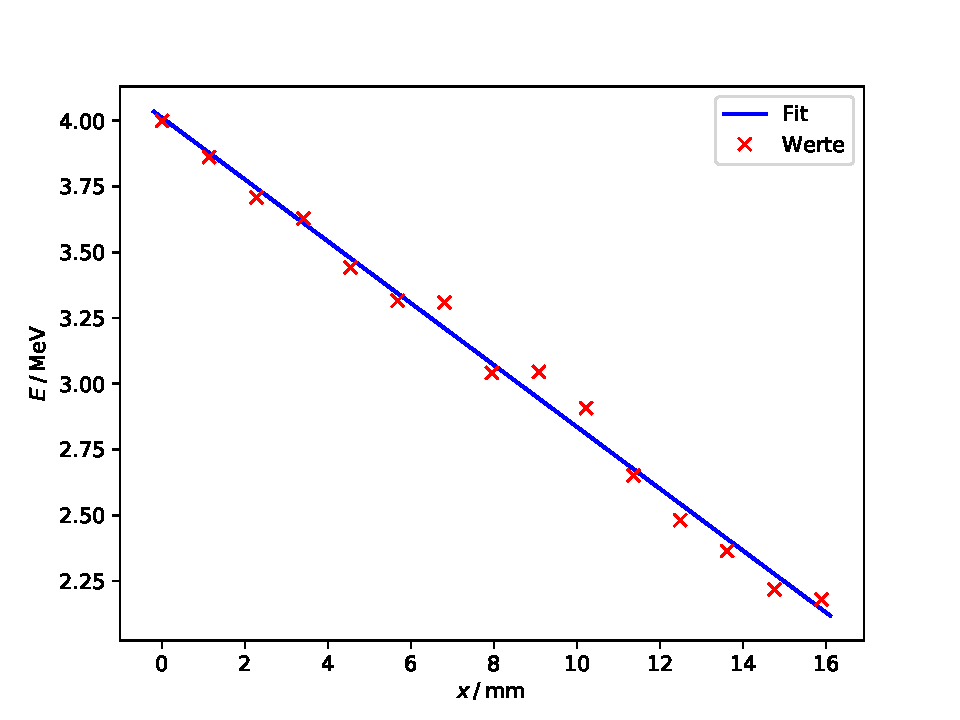
\includegraphics[width=\textwidth]{Plots/energie23mm.pdf}
  \caption{$E$-$x$-Diagramm zur Bestimmung des Energieverlustes von $\symup{\alpha}$-Strahlung}
  \label{fig:energie23mm}
\end{figure}

Eine lineare Regression $f(x) = -c \cdot x + d$ ergibt
\begin{align*}
  c &= \SI{0,118(3)}{\MeV \per \mm} = \frac{\symup{d} E}{\symup{d} x} \\
  d &= \SI{4,01(3)}{\MeV}.
\end{align*}

\subsubsection{Messung 2 - $d = \SI{24}{\mm}$ \label{sec:24mm}}

In Tabelle \ref{tab:reich24mm} befinden sich die aufgenommenen Messwerte.
\input{Text/Tabellen/reich24mm.tex}

Der effektive Abstand $x$ zwischen Strahler und Detektor ergibt sich wieder aus Gleichung \eqref{eqn:xeff}.
In Abbildung \ref{fig:reich24mm} sind die Zählraten in Abhängigkeit vom effektiven Abstand aufgetragen.
\begin{figure}[H]
  \centering
  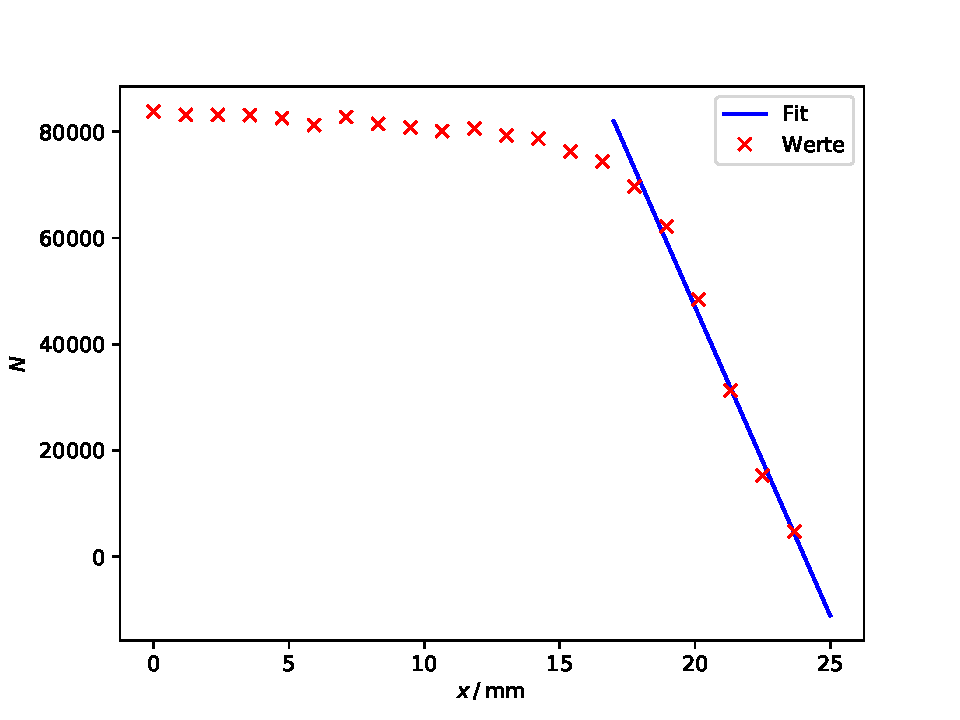
\includegraphics[width=\textwidth]{Plots/reich24mm.pdf}
  \caption{$N$-$x$-Diagramm zur Bestimmung der mittleren Reichweite von $\symup{\alpha}$-Strahlung}
  \label{fig:reich24mm}
\end{figure}

Eine lineare Regression $f(x) = -a \cdot x + b$ ergibt
\begin{align*}
  a &= \SI{1,16(6)e4}{\per \mm} \\
  b &= \SI{2,8(1)e5}{}
\end{align*}

Die maximale Zählrate beträgt hier ungefähr $N_\text{max} = \SI{81826}{}$. Für die mittlere Reichweite ergibt sich nach Gleichung \eqref{eqn:rm} und \eqref{eqn:errrm} zu
\begin{equation*}
  R_m = \SI{20,5(15)}{\mm}.
\end{equation*}

Der mittleren Reichweite entspricht nach Gleichung \eqref{eqn:e} und \eqref{eqn:erre} einer Energie von
\begin{equation*}
  E_{\symup{\alpha}} = \SI{3,5(2)}{\MeV}.
\end{equation*}

In Abbildung \ref{fig:energie24mm} ist die Energie gegen den effektiven Abstand aufgetragen.
\begin{figure}[H]
  \centering
  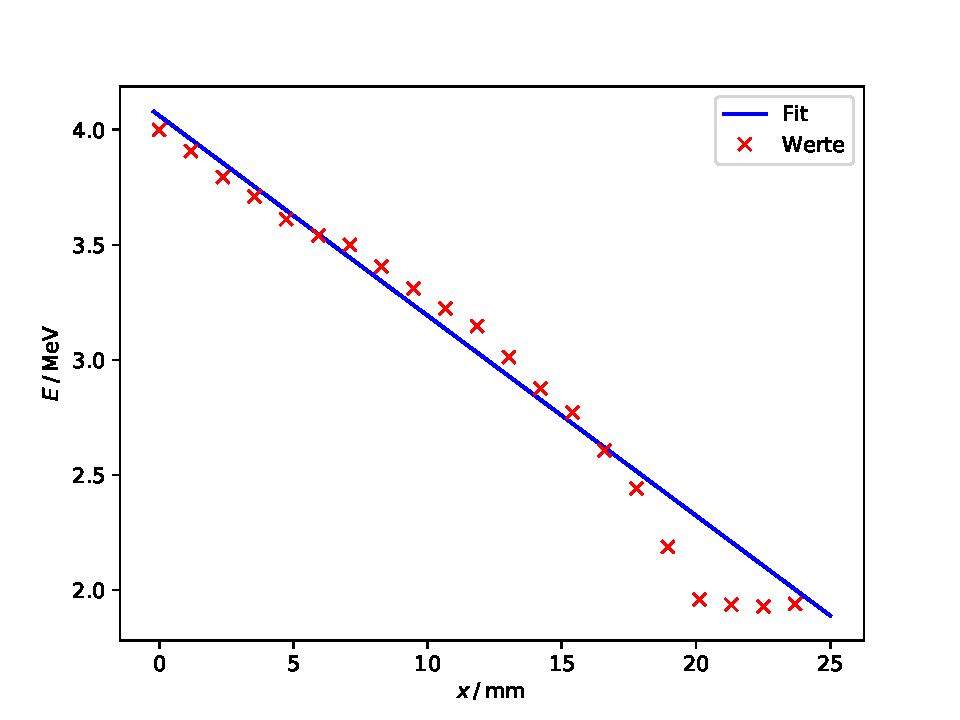
\includegraphics[width=\textwidth]{Plots/energie24mm.pdf}
  \caption{$E$-$x$-Diagramm zur Bestimmung des Energieverlustes von $\symup{\alpha}$-Strahlung}
  \label{fig:energie24mm}
\end{figure}

Eine lineare Regression $f(x) = -c \cdot x + d$ ergibt
\begin{align*}
  c &= \SI{0,087(4)}{\MeV \per \mm} = \frac{\symup{d} E}{\symup{d} x} \\
  d &= \SI{4,06(4)}{\MeV}.
\end{align*}

\subsection{Statistik des radioaktiven Zerfalls}

In Tabelle \ref{tab:vert} befinden sich aufgenommenen Messwerte. Das Messintervall beträgt $\SI{10}{\s}$.
\input{Text/Tabellen/vert.tex}

In Abbildung \ref{fig:vert} sind die Zerfallsraten als Histogramm aufgetragen. Zum Vergleich sind die Gauß- und Poissonverteilung ebenfalls aufgetragen.
\begin{figure}[H]
  \centering
  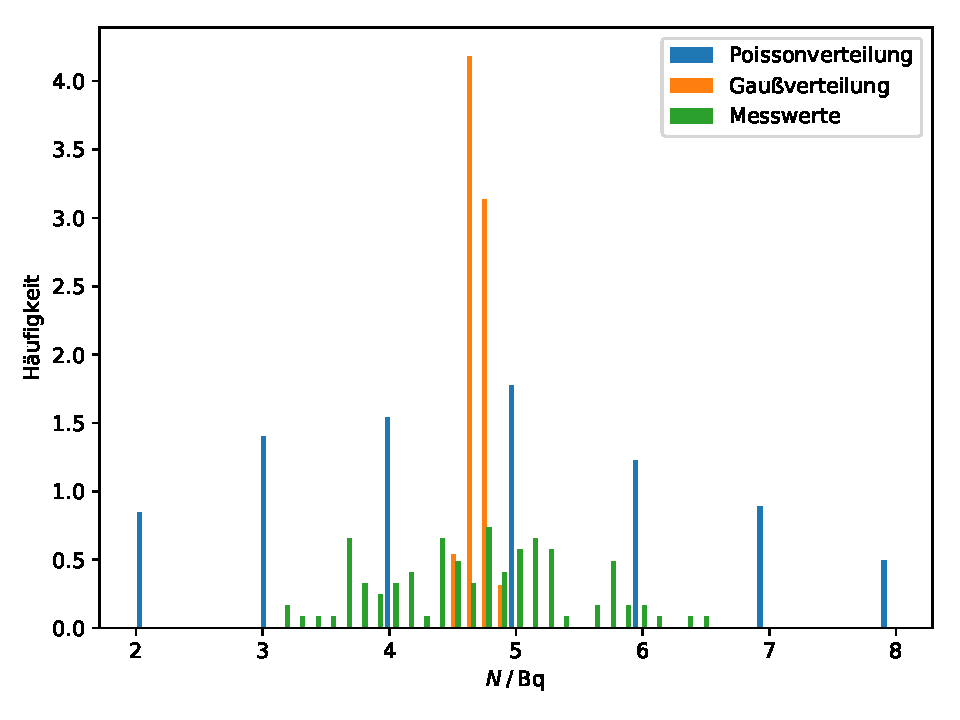
\includegraphics[width=\textwidth]{Plots/vert.pdf}
  \caption{Histogramm zum Vergleich der gemessenen Zerfallsraten mit der Gauß- und Poissonverteilung}
  \label{fig:vert}
\end{figure}

Der Mittelwert und die Standardabweichung der Werte aus Tabelle \ref{tab:vert} ergeben sich aus Gleichung \eqref{eqn:mit} und \eqref{eqn:sta}
\begin{align}
  \bar{N} &= \frac{1}{100} \sum_{i=1}^{100} N_i
  \label{eqn:mit} \\
  \sigma_{\bar{N}} &= \sqrt{\frac{1}{100 (100 - 1)} \sum_{i=1}^{100} (N_i - \bar{N})^2}.
  \label{eqn:sta}
\end{align}

Somit beträgt der Mittelwert
\begin{equation*}
  \bar{N} = \SI{4,68(7)}{\becquerel}.
\end{equation*}
